\documentclass[a4paper,12pt]{article}

%%% Работа с русским языком % для pdfLatex
\usepackage{cmap}					% поиск в~PDF
\usepackage{mathtext} 				% русские буквы в~фомулах
\usepackage[T2A]{fontenc}			% кодировка
\usepackage[utf8]{inputenc}			% кодировка исходного текста
\usepackage[english,russian]{babel}	% локализация и переносы
\usepackage{indentfirst} 			% отступ 1 абзаца
\usepackage{gensymb}				% мат символы?

%%% Работа с русским языком % для XeLatex
%\usepackage[english,russian]{babel}   %% загружает пакет многоязыковой вёрстки
%\usepackage{fontspec}      %% подготавливает загрузку шрифтов Open Type, True Type и др.
%\defaultfontfeatures{Ligatures={TeX},Renderer=Basic}  %% свойства шрифтов по умолчанию
%\setmainfont[Ligatures={TeX,Historic}]{Times New Roman} %% задаёт основной шрифт документа
%\setsansfont{Comic Sans MS}                    %% задаёт шрифт без засечек
%\setmonofont{Courier New}
%\usepackage{indentfirst}
%\frenchspacing

%%% Дополнительная работа с математикой
\usepackage{amsfonts,amssymb,amsthm,mathtools}
\usepackage{amsmath}
\usepackage{icomma} % "Умная" запятая: $0,2$ --- число, $0, 2$ --- перечисление
\usepackage{upgreek}

%% Номера формул
%\mathtoolsset{showonlyrefs=true} % Показывать номера только у тех формул, на которые есть \eqref{} в~тексте.

%%% Страница
\usepackage{extsizes} % Возможность сделать 14-й шрифт

%% Шрифты
\usepackage{euscript}	 % Шрифт Евклид
\usepackage{mathrsfs} % Красивый матшрифт

%% Свои команды
\DeclareMathOperator{\sgn}{\mathop{sgn}} % создание новой конанды \sgn (типо как \sin)
\DeclareMathOperator{\rg}{\mathop{rg}}
\DeclareMathOperator{\Rg}{\mathop{Rg}}
\DeclareMathOperator{\im}{\mathop{Im}}
%\DeclareMathOperator{\dim}{\mathop{dim}}
\usepackage{csquotes} % ещё одна штука для цитат
\newcommand{\pd}[2]{\ensuremath{\cfrac{\partial #1}{\partial #2}}} % частная производная
\newcommand{\abs}[1]{\ensuremath{\left|#1\right|}} % модуль
\renewcommand{\phi}{\ensuremath{\varphi}} % греческая фи
\newcommand{\pogk}[1]{\!\left(\cfrac{\sigma_{#1}}{#1}\right)^{\!\!\!2}\!} % для погрешностей

% Ссылки
\usepackage{color} % подключить пакет color
% выбрать цвета
\definecolor{BlueGreen}{RGB}{49,152,255}
\definecolor{Violet}{RGB}{120,80,120}
% назначить цвета при подключении hyperref
\usepackage[unicode, colorlinks, urlcolor=blue, linkcolor=blue, pagecolor=blue, citecolor=blue]{hyperref} %синие ссылки
%\usepackage[unicode, colorlinks, urlcolor=black, linkcolor=black, pagecolor=black, citecolor=black]{hyperref} % для печати (отключить верхний!)


%% Перенос знаков в~формулах (по Львовскому)
\newcommand*{\hm}[1]{#1\nobreak\discretionary{}
	{\hbox{$\mathsurround=0pt #1$}}{}}

%%% Работа с картинками
\usepackage{graphicx}  % Для вставки рисунков
\graphicspath{{images/}{images2/}}  % папки с картинками
\setlength\fboxsep{3pt} % Отступ рамки \fbox{} от рисунка
\setlength\fboxrule{1pt} % Толщина линий рамки \fbox{}
\usepackage{wrapfig} % Обтекание рисунков и таблиц текстом
\usepackage{multicol}

%%% Работа с таблицами
\usepackage{array,tabularx,tabulary,booktabs} % Дополнительная работа с таблицами
\usepackage{longtable}  % Длинные таблицы
\usepackage{multirow} % Слияние строк в~таблице
\usepackage{caption}
\captionsetup{labelsep=period, labelfont=bf}

%%% Оформление
\usepackage{indentfirst} % Красная строка
%\setlength{\parskip}{0.3cm} % отступы между абзацами
%%% Название разделов
\usepackage{titlesec}
\titlelabel{\thetitle.\quad}
\renewcommand{\figurename}{\textbf{Рис.}}		%Чтобы вместо figure под рисунками писал "рис"
\renewcommand{\tablename}{\textbf{Таблица}}		%Чтобы вместо table над таблицами писал Таблица
\usepackage{enumitem}
\setlist{nolistsep}
\usepackage{verbatim}

%%% Теоремы
\theoremstyle{plain} % Это стиль по умолчанию, его можно не переопределять.
\newtheorem{theorem}{Теорема}[section]
\newtheorem{proposition}[theorem]{Утверждение}
\newtheorem{predlog}{Предложение}[section]
\newtheorem{lemma}{Лемма}[section]

\theoremstyle{definition} % "Определение"
\newtheorem{definition}{Определение}[section]
\newtheorem{corollary}{Следствие}[theorem]
\newtheorem{problem}{Задача}[section]

\theoremstyle{remark} % "Примечание"
\newtheorem*{nonum}{Решение}
\newtheorem{zamech}{Замечание}[theorem]

%%% Правильные мат. символы для русского языка
\renewcommand{\epsilon}{\ensuremath{\varepsilon}}
\renewcommand{\phi}{\ensuremath{\varphi}}
\renewcommand{\kappa}{\ensuremath{\varkappa}}
\renewcommand{\le}{\ensuremath{\leqslant}}
\renewcommand{\leq}{\ensuremath{\leqslant}}
\renewcommand{\ge}{\ensuremath{\geqslant}}
\renewcommand{\geq}{\ensuremath{\geqslant}}
\renewcommand{\emptyset}{\varnothing}

%%% Для лекций по инфе
\usepackage{alltt}
\newcounter{infa}[section]
\newcounter{num}
\definecolor{infa}{rgb}{0, 0.2, 0.89}
\definecolor{infa1}{rgb}{0, 0.3, 1}
\definecolor{grey}{rgb}{0.5, 0.5, 0.5}
\newcommand{\tab}{\ \ \ }
\newcommand{\com}[1]{{\color{grey}\##1}}
\newcommand{\num}{\addtocounter{num}{1}\arabic{num}\tab}
\newcommand{\defi}{{\color{infa}def}}
\newcommand{\ini}{{\color{infa}in}}
\newcommand{\rangei}{{\color{infa}range}}
\newcommand{\fori}{{\color{infa}for}}
\newcommand{\ifi}{{\color{infa}if}}
\newcommand{\elsei}{{\color{infa}else}}
\newcommand{\printi}{{\color{infa1}print}}
\newcommand{\maxi}{{\color{infa}max}}
\newcommand{\classi}{{\color{infa}class}}
\newcommand{\returni}{{\color{infa}return}}
\newcommand{\elifi}{{\color{infa}elif}}
\newenvironment{infa}[1]{
	
	\vspace{0.5cm}
	\addtocounter{infa}{1}%
	\noindent{\large \textbf{Программа №\thesection.\arabic{infa}}}\textbf{<<#1>>}%
	\begin{alltt}%
	}{\end{alltt}
	\setcounter{num}{0}
	\vspace{0.1cm}}
%Пример кода:
%\begin{infa}{Поразрядная сортировка}
%	\ \num \defi count_sort(a):\tab \com{определяет нашу функцию}
%	\ \num \tab m = \maxi(a)+1
%	\ \num \tab q = [0]*m
%	\ \num \tab \fori x \ini a:
%	\ \num \tab \tab q[x] += 1
%	\ \num \tab pos = 0
%	\ \num \tab \fori x \ini q:
%	\ \num \tab \tab \fori i \ini \rangei(q[x]):
%	\ \num \tab \tab \tab a[pos] = x
%	\num \tab \tab \tab pos += 1
%\end{infa}

\newcommand{\game}[1]{\begin{center}\textbf{#1}\end{center}}

\begin{document}
\game{Игра по типу сороконожки}
Двое играют в следующую простую разновидность покера.

Сначала первый игрок берёт карту из колоды (карта с равными вероятностями может быть красной или чёрной), смотрит на неё. После чего может вскрыться или удвоить ставку. Если ставка удвоена, то второй либо просит показать карту, либо сбрасывает её обратно в колоду. Если карта чёрная, то первый платит второму (1 до удвоения или 2 после удвоения), если красная, то, наоборот, второй платит первому 1 или 2 в зависимости наличия удвоения. Если карта сброшена, то второй игрок платит первому рубль.

\begin{enumerate}
	\item \textbf{Как выглядит дерево этой игры?}\\
	\textit{Ответ:\\
	\begin{figure}[h]
		\centering
		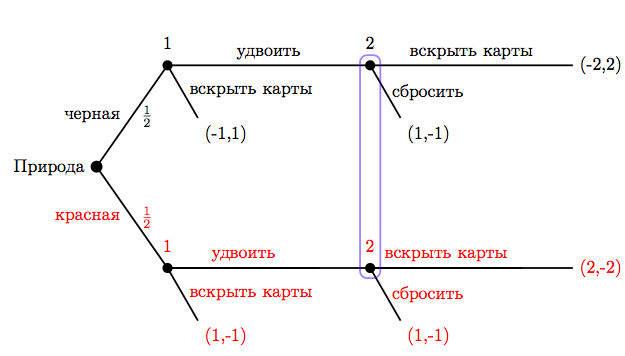
\includegraphics[width=0.7\linewidth]{wrq-xCfeEeaNKg4a0RSP6Q_fcfea7413b8afe48a6a40361b7de01b6_w06_test2}
		\caption{}
		\label{fig:wrq-xcfeeeankg4a0rsp6qfcfea7413b8afe48a6a40361b7de01b6w06test2}
	\end{figure}
	Вначале природа выбирает, какая карта выпадет. Первый игрок знает о том, какая карта ему досталась, и решает, удвоить ставку или нет. В свою очередь, второй игрок не знает, какая карта у первого, и решает, вскрываться или нет. Поэтому у второго есть информационное множество.}
	\item Предположим, что оба игрока используют смешанные стратегии в управляемых им вершинах, кроме того, второй игрок верит в то, что находится в верхней вершине с вероятностью $\omega$. Вероятности и веры согласованы между собой. Допустим, что первый игрок с ненулевой вероятностью удваивает в обоих случаях, и данные профили стратегий находятся в равновесии.
	
	\textbf{Какое соотношение на веру $\omega$ второго игрока о нахождении его в верхней вершине выполнено?}\\
	\textit{Ответ: $$2\omega-2(1-\omega) = -1$$ Если второй игрок верит, что он находится в верхней вершине с вероятностью $\omega$, и в нижней с вероятностью $1-\omega$ и использует смешанное равновесие, то ему всё равно, как сходить в этом случае. Ожидаемый выигрыш от применения стратегии <<вскрыть карты>> равен $2\omega-2(1-\omega)$, от стратегии сбросить - $-1$.}
	\item \textbf{Чему равна вера $\omega$ второго игрока о нахождении его в верхней вершине?}\\
	\textit{Ответ: из предыдущего $\omega = 0.25$.}
	\item Будем считать, что мы находимся в предположениях задачи 2. Пусть вероятность вскрыть карты у второго игрока равна $\gamma$, а вероятности повысить удвоить у первого игрока равны $\alpha$ при чёрной карте и $\beta$ при красной карте (см. рисунок внизу после заданий).
	\begin{figure}[h!]
		\centering
		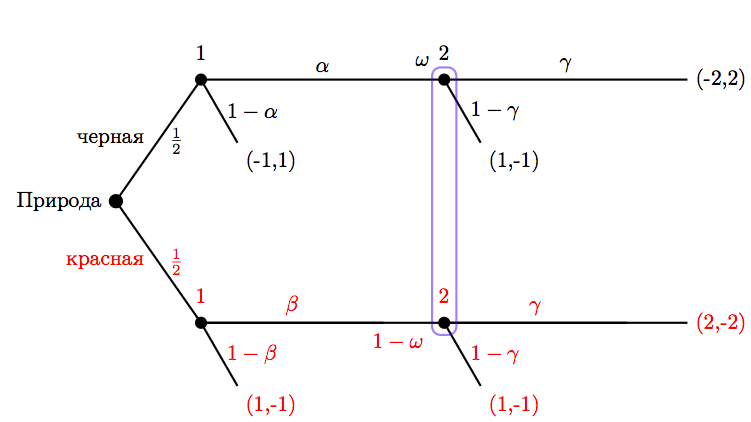
\includegraphics[width=0.7\linewidth]{wVBHNifgEeak5wpS_JmWWw_6fbbaac5a5e6813956346cf1ffe95c35_w06_test5}
		\caption{}
		\label{fig:wvbhnifgeeak5wpsjmwww6fbbaac5a5e6813956346cf1ffe95c35w06test5}
	\end{figure}

	\textbf{При каком $\gamma$ первый игрок будет смешивать свои стратегии при чёрной и красной картах?}\\
	\textit{Ответ: $$(2/3, 0)$$ Первый игрок будет смешивать свои стратегии, если ожидаемый выигрыш от использования стратегий <<удвоить>> или <<вскрыть>> будет одинаковым. Поэтому мы получаем равенства: $-1=-2\gamma+(1-\gamma)$ для чёрной карты и $1=2\gamma+(1-\gamma)$ для красной карты, откуда $\gamma=2/3$ в первом случае и $\gamma=0$ во втором.}
	\item Исходя из предыдущей задачи, мы получаем, что первый игрок не будет смешивать свои стратегии в обоих случаях. Так как мы рассматриваем случай, когда он удваивает в каждом из случаев с ненулевой вероятностью логично предположить, что $\gamma=2/3$. \textbf{Какие значения принимают $\alpha$ и $\beta$ (Напоминаем, что вера $\omega$ второго игрока должна быть согласована с вероятностями попасть в соответствующую вершину.)}\\
	\textit{Ответ: $\alpha = 1/3$ (объяснение ниже). }
	\item \textit{$\beta = 1$. Если $\gamma=2/3$, то $\beta = 1$, так как первому игроку в случае удачной карты будет выгоднее удвоить ставку. Так как вера $\omega = 1/4$, то мы имеем соотношение: $\frac{1/2\alpha}{1/2\beta} = \frac{\omega}{1-\omega}$, откуда $\alpha = 1/3$.}
\end{enumerate}
\newpage
\game{Игра <<Координация>>}
Рассмотрим игру <<Координация>>, изменив начальные данные. Напомним формулировку.

Играют два игрока, у каждого есть две стратегии "выяснить информацию" или "понадеяться на второго". Матрица выигрышей выглядит следующим образом:
$$
\begin{pmatrix}
			&\text{выяснить}&\text{понадеяться}\\
	\text{выяснить}&(1-c, 1-c)& (1-c, 1)\\
	\text{понадеяться}&(1, 1-c)&(0, 0)\\
\end{pmatrix}
$$
Значение $c$ заранее неизвестно. Для первого игрока оно равномерно распределено на отрезке $[0, 1/2]$, для второго - на отрезке $[0, 2/3]$ (на лекции отрезки у игроков были одинаковы). Каждый игрок знает своё значение c и распределение второго.

Положим $C_1$ (соответственно, $C_2$) - те значения $c$, при которых первый (соответственно, второй) игрок выясняет информацию (будем считать, что эти множества измеримы). Кроме того, обозначим через $c_1$ и $c_2$ реальные значения издержек для первого и второго игроков.

\begin{enumerate}
	\item\textbf{В каком случае первый игрок будет выяснять информацию? (то есть он не захочет понадеяться на второго игрока).}\\
	\textit{Ответ: $1-c_1\geq \mathcal{P}(C_2)$. Выигрыш первого игрока от применения стратегии <<выяснить>> равно $1-c_1$, от <<понадеяться>> - $\mathcal{P}(C_2)$ (так как это в точности те случаи, когда второй выясняет).}
	\item В условиях предыдущей задачи предположим, что оба игрока выбрали поведения для каждого значения параметров $(c_1, c_2)$ так, что
	
	1) вероятности $\mathcal{P}_1=\mathcal{P}(C_1)$ и $\mathcal{P}_2=\mathcal{P}(C_2)$ определены и не равны 0 или 1;
	
	2) система находится в равновесии, то есть при данном выборе поведений никакому игроку невыгодно изменять свою стратегию ни для какого значения $c_1$, $c_2$.
	
	\textbf{Какие соотношения в этом случае гарантированно выполняются?}\\
	\textit{Ответ: из предыдущей задачи следует, что первый игрок выясняет информацию только в том случае, если $1-c_1\geq \mathcal{P}(C_2)=P_2\Leftrightarrow c_1\leq 1-\mathcal{P}_2$. Аналогично для второго игрока.}
	\item Из соотношений, выведенных в предыдущей задаче, получите систему на $\mathcal{P}_1$ и $\mathcal{P}_2$ и решите её. \textbf{Какие получатся значения?}\\
	\textit{Ответ: $\mathcal{P}_1 = 1/2$.}
	\item \textit{$\mathcal{P}_2 = 3/4$. Из распределений и отношения площадей.}
	\item \textbf{Чему равно пороговое значение издержек при котором будет безразлично: искать решение самому или понадеяться на соседа?}\\
	\textit{Ответ: $\hat{c}_1 = 1/4$, $\hat{c}_2 = 1/2$. Из распределений + п. 2.}
\end{enumerate}

\end{document}